\section{Methods}
\label{sec:methods}

In general the inpainting problem can be seen as a Maximum Likelihood Estimation (MLE) problem where the objective is to fill the missing pixels with most likely values, given the observed data \cite{fadili2009inpainting}. We represent the known values of the image through sparse encoding and during the process, infer pixel values at the locations of the unknown pixels, using the characteristics of the encoding basis. Popular bases include Discrete Cosine Transforms (DCT), Haar wavelets etc. which demonstrate favorable qualities for image encoding as they exhibit characteristics similar to generic image features. To achieve the sparse encoding we use the matching pursuit algorithm which serves to meet the following criterion 
\begin{align*}
   z^* &\in \arg\max_{z} \Vert\mathbf{M}(\mathbf{x}-\mathbf{U}\mathbf{z}) \Vert_2 \\
   		& s.t. \Vert z_0\Vert  \leqslant K
\end{align*}
where $\mathbf{M}$ is the masking matrix, $\mathbf{x}$ is the observed pixels, $\mathbf{U}$ is the dictionary matrix and $\mathbf{z}$ are its sparse coefficients. \cite{CIL2015}



Inpainting through sparse coding relies on inferring unknown values based on the impact the known pixels incur on the chosen basis. Therefore, for a given genre of images it is advantageous to utilize a custom dictionary which can easily encode the given genre's typical image characteristics. For example  in \cite{elad2005simultaneous}, curvelets were demonstrated to be specifically efficient at encoding cartoon images.

So far in the technique mentioned, the image is divided into individual patches on which the sparse encodings are found. This approach disregards the spatial distribution of the occlusions and is hence sensitive to images where certain patches contain little known information. In \cite{criminisi2004region} a method is proposed which first ranks mask pixels with a (local) confidence criterion that favors pixels whose neighbourhood contain relevant structure. Then, dense information from the boundary patches of the masked regions are propagated throughout the occluded region. Inspired by this work, we pursue here two ways of propagating valuable image information beyond the boundaries of one patch: Valuable Information Propagation (VIP) and Confidence Blending (CB). This section is finalized with a description of our learning scheme for dictionaries.

\subsection{Valuable Information Propagation (VIP)}
To tackle the issue of densely populated masks, one of our approaches was to infer information from the surrounding, better known neighbours. The patches are ranked by a confidence criterion; we employ here the proportion of known pixel values within a patch, as a quality measure. Propagating information from better to poorer patches is then done by performing inpainting on an imaginary patch which is the concatenation of the poor patch's boundaries and its corresponding better neighbour. Once this imaginary patch's pixels have been inferred, parts of the poorer neighbour's boundary missing pixels are chosen at random, and updated. This step allows for the propagation of information from the better neighbouring patch, while also reserving some of the final reconstruction influence for the poorer patch itself. The proportion of the masked pixels updated during this step is controlled by a parameter $\epsilon \in \left] 0,1 \right[$, which controls the amount of information propagated from the neighbour. The boundary width i.e. the band of pixels that make up the boundary is also parameterized as a function of the patch size. This value determines the autonomy that a given poor pixel has over its final image reconstruction. The algorithm works as follows

%   
%
%\vspace{-0.2cm}%
%\alglanguage{pseudocode}
%\begin{algorithm}[h]
%\small
%\caption{Valuable Information Propagation}
%\label{Algorithm:VIP}
%\begin{algorithmic}[1]
%\Create{$\mathbf{Descending patch quality order}$}{vector $Rank$}
%  %%  \LineComment{\emph{Quick check if $x$ is in mCBF}}
%    \For {$i = 1 \to length(Rank)$}
%            %%\If {$mCBF.C_{f_i(x)\%N}$ == 0}
%                %%\State \textbf{return}
%            %%\EndIf
%	SparseCoding of patch $i$
%	update mask vector in  \mathbf{M} and image vector in  \mathbf{X} corresponding to patch i
%	
%	    \For {$j = 1 \to #Neighbours$}
%		\If {$#Masked values_j}$ >= \mathbf{threshold}}
%               	 \State {Perform information propagation from i to j}
%			update mask and pixel values of j
%	            \EndIf
%	    \EndFor
%    \EndFor
%    
%\Statex
%\end{algorithmic}
%  \vspace{-0.4cm}%
%\end{algorithm}

\subsection{Confidence Blending (CB)}
Inpainting by means of sparse coding operates on image patches, that is, the missing pixels are filled patch by patch. To introduce redundancy, we suggest that these image patches overlap by a certain degree. This way, it is possible to combine suggestions for missing pixels from different patches. Consider for example patches of size $p\times p$ that overlap each other by $o=1-p/f$, $f=2$. Then every pixel of the input image (except for those within the border of width $o$) will be covered by 4 patches. This situation is depicted in figure \ref{fig:overlapping_patches}. Hence, the reconstruction is 4-way redundant. Higher redundancy can be achieved for higher $f$, but this comes at a higher computational cost since the number of patches increases quadratically in $f$. Note that the overlapping regions are of size $p/f$, we call them \textit{patchlets}.

\begin{figure}[b]
   \centering
	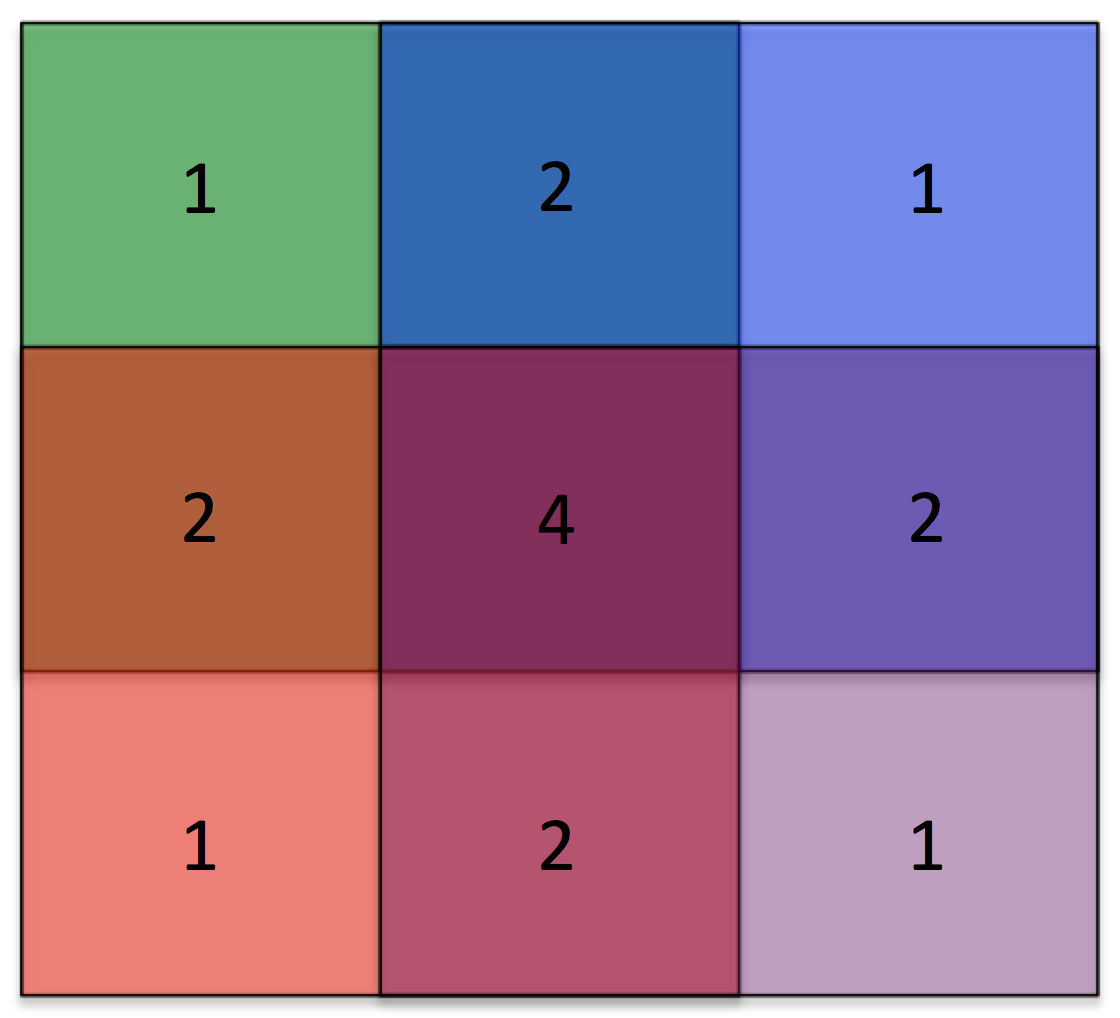
\includegraphics[width=.5\columnwidth]{graphics/overlapping_patches.png}%
	\caption{Image with four patches with $o=p/2$. The numbers indicate the number of overlapping patchlets in each position.
	\label{fig:overlapping_patches}
	}
\end{figure}

We refer to \textit{blending} when patches are combined. The simplest way of blending is to calculate a weighted average of the patchlets $p_i$ for $i\in\{1,2,3,4\}$ with a fixed weight $w_i$: $p=\sum_i w_i \cdot p_i/\sum_i w_i$ (where ``$+,\cdot$" denote the pixel-wise addition and multiplication of patch-sized matrices respectively). Our experiments show the that this has a very beneficial effect on the visually perceived result because small artifacts are evened out.

In our method, we opted for a dynamic weighing that aims, before anything, at improving the overall visual perception. 
The human visual system in general is very sensitive to discontinuities (cracks). Hence, it is preferable to avoid a reconstruction that exhibits strong gradients in luminosity at the border of an inpainted area.\footnote{Of course, it may happen that edges in the image coincide with a mask boundary. But the chance that these correlate with the boundary of typical masks is in general small.}

This motivates our \textit{confidence blending} (CB) method, which operates with weights that take into account the luminosity gradients across mask borders. If $M$ denotes the mask, $\partial M$ its boundary and $I_R$ the reconstructed image, then a confidence $c(j) \in [0,1]$ can be calculated for every pixel $j\in \partial M$:
\begin{align*}
c_1(j) &= 1-\kappa|\nabla M(j) \cdot \nabla I_R(j)|\\
c_2(j) &= 1-\kappa \Vert\nabla I_R(j)\Vert_2\\
j &\in \partial M
\end{align*}
The confidence $c_1$ expresses how strongly the image gradients on $\partial M$ correlate with the mask borders. Low values of $c_1$ indicate that the mask boundary coincides with an edge found in the reconstructed image. Note that $\kappa$ is used to scale the gradient expression such that it maps to the range $[0,1]$. $c_2$ is a simpler confidence measure that ignores the gradient directions. In our implementation, we prefer $c_2$ over $c_1$ because it gives only slightly worse results while being faster.

Next, these point-wise confidence observations along $\partial M$ can be assembled into a weight $W$. A convolution with a Gaussian kernel\footnote{Our implementation uses kernel size $k=3$ and $\sigma=1$} helps to spread the information from the border to the inner of the mask. Pixels outside the mask are ignored.

Repeating this for the $f^2$ reconstructed images $I_{R_i}$ yields masks $W_i$, with which weighted blending can be performed as already done for the simple scheme.

Blending improves the perceived quality because the support is increased for the filled-in pixels: every patch covers a different part of the image.



\subsection{Dictionary learning}
The dictionary $U$ plays a decisive role both in terms of reconstruction quality and run-time. It further has a strong impact on the sparsity of the encoding that is possible with it. Hence it is important to elaborate on the particular choice of the dictionary. In the following we present our methods how to learn dictionaries. For a definition of terms such as \textit{dictionary} or \textit{atoms}, and a description of how sparse coding operates on these, we refer to \cite{CIL2015}.

The objective is to assemble a lightweight dictionary on the space of $p \times p$ patches $\mathbb{E}$ such that it is still able to accurately encode image patches. Motivated by experiments, we decided to rely on under-complete dictionaries for $p=16$ pixels that are composed of 64 atoms (25\% of $\dim\mathbb{E}$). To train such a dictionary, we suggest to apply the approximate \textit{K-SVD} algorithm on a \textit{training data} customized for our purposes. Particular attention has to be paid for the \textit{initialization} of the learning process \cite{CIL2015}. 

\mypar{K-SVD algorithm}
The algorithm takes a training set of patches $X = (p_i, \ldots p_n), p_i \in \mathbb{E}$ and learns a dictionary $U$, starting from an initial dictionary $U_0$ and iteratively modifying $U$ to represent $X$ in an efficient way. \cite{CIL2015} For all our dictionaries, we used this algorithm with 15 iterations, using the same training data set.

\mypar{Construction of training set}
The dictionary being under-complete, loss of information is inevitable when decoding an image. However, the choice of the dictionary should reflect the characteristics of images for which it is targeted in the best possible way. 

We constructed our test set by extracting $16\times 16$ patches from 36 randomly selected photographs of size $512\times 512$ pixels, showing mostly real-life scenes with varying characteristics. To this pool of patches we applied Principal Component Analysis (PCA) on these patches to find the most significant 64-dimensional subspace $\eta_{PCA}\in\mathbb{E}$ that preserves the characteristics contained in the patches the best. The patches then are projected onto $\eta_{PCA}$, which results in the actual data-set $X$ that is used for learning. The complete process of dictionary learning operates within $\eta_{PCA}$, safely ignoring the less relevant directions of $\mathbb{E}$.

\mypar{Initialization}
K-SVD requires an initial dictionary $U_0$, starting from which it optimizes greedily. We observed that the choice of $U_0$ has a strong influence on the resulting dictionary $U$. To better control over this step, we implemented 3 different ways to initialize the learning process and compared them with each other:
\begin{itemize}
   \item Fixed dictionary: with this approach, the dictionary is initialized with a particular dictionary, such as a 64-atom DCT dictionary, or the 64 significant vectors obtained by applying PCA to the training set.  
   \item $K$-means initialization: here, we initialize the dictionary based on the training data set $X$. We first center and normalize the training data, after which we apply the $K$-means algorithm with $K$=64 based on the euclidean norm, and use the normalized 64 centroids as initializing atoms. To improve the robustness of the $K$-mean algorithm, we applied the algorithm 10 times and chose the result which had the smallest mean pairwise-distance with other clustering. 
   \item Random initialization: A randomly-generated initialization of $U$ is used as a reference. 
\end{itemize}

